\chapter{Related Work}
There is a large body of active research on using the hand as an input modality
for HCI.  A gestural input
pipeline can be broken down into several sequential modules: sensors, hand
tracking, feature extraction, gesture recognition, and user interfaces.
I discuss the related work in each module.

\section{Sensors}
The first step in the pipeline is having sensors that capture the hand movements
and configurations, converting analog signals to digital signals. First attempts
to solve this problem resulted in mechanical devices that directly measure hand
joint angles and spatial positions. This group is best represented by the
glove-based approaches using devices such us CyberGloves \cite{fels09} and
Powergloves \cite{kadous02}. However, wearing gloves makes gesturing more
cumbersome, and many efforts have been made to make the gloves more
light-weight, for example, by using Bluetooth wireless data transmission (e.g.,
CyberGove II). To further reduce the bulkiness of the gloves, people use colored
markers on the fingers \cite{mistry09} or colored gloves with no electronics \cite{Wang09}, and use RGB
cameras and computer vision techniques to interpret gestures. However, by
requiring the user to wear something extra still hinders the acceptance of
such devices as ``everyday'' natural interaction interfaces. 

The most non-obtrusive way to capture the hand is bare-hand tracking. Shin et
al. \cite{shin04} use stereo RGB cameras to extract the hand from background
based on the skin color. One limitation of RGB cameras is that they are very sensitive to lighting
conditions. This prompted researchers to look into other types of cameras. Oka et al. 
\cite{Oka02} use thermal imaging for hand segmentation under complex
background and changing light, relying on the condition that a hand's
temperature is almost always distinct from the background. Their approach does
not detect finger contact with the surface. Larson et al. \cite{larson11}
improve on this method to detect the finger contact by using
the heat transferred from a user's hand to the surface for touch-based gestures.
However, in order to detect the heat trace, the user has to drag the fingers a
bit instead of just touching. This may be a small departure from what users
would expect as ``natural'' based on their experience in the physical world.

Thermal imaging measures radiation emitted by objects in the
\textit{far}-infrared (F-IR) spectrum. There are other well-known ``IR-imaging''
techniques used in the HCI community which use devices that operate in the \textit{near}-infrared (N-IR) spectrum.
N-IR is employed in some fairly recent interactive tabletop surfaces and depth
cameras. A number of projects in the HCI community have used IR for tabletop
interaction by detecting multi-touch gestures using an under mounted
camera and an illumination source. An example of this is Microsoft's 
Surface. Recently, multi-touch phones and tablets have become more and more ubiquitous. These devices
are based on capacitive touch sensitive screens. Touch-based devices are
becoming more and more mature, however the kind of gestures one can use are still
limited. The gestures are usually limited in 2D space with one or multiple
fingers. 

Going beyond the limitation of touch-only gestures, 
depth sensing input devices such as the Kinect sensor and the Leap Motion
Controller open up the realm for gesturing in 3D space. The Kinect sensor
contains a depth sensor, a color camera, and a four-microphone array that
provide full-body 3D motion capture, facial recognition, and voice recognition
capabilities~\cite{zhang12}. The first generation of the sensor
uses structured light principle for depth sensing.
The color stream has a resolution of $640\times
480$px at 30Hz or $1280\times960$px at 12Hz.  The depth sensing video stream has a resolution of $640\times 480$ pixels at
30Hz\footnote{\url{http://msdn.microsoft.com/en-us/library/jj131033.aspx}}. 
With default range, the Kinect sensor (version one) has a depth sensing range limit of about 0.8m - 4m.
The random error of its depth measurements increases quadratically with
increasing distance from the sensor and ranges from a few millimeters at 0.5m distance to about 4cm
at the maximum range of 5m~\cite{khoshelham2011}. The newer version of Kinect
uses a 1080p ($1920\times 1080$px) wide-angle time-of-flight
camera\footnote{\url{http://en.wikipedia.org/wiki/Xbox_One}}, and has greater
accuracy with three times the fidelity over the older version~\cite{kinect14}.
In stead of full-body tracking, the Leap Motion Controller has a
smaller observation area and specializes in hand tracking with higher
resolution.
It uses two monochromatic IR cameras and three infrared LEDs, and observes a
roughly hemispherical area, to a distance of about 1m~\cite{leapmotion14}. It
can track all 10 fingers up to 1/100th of a
millimeter\footnote{\url{https://www.leapmotion.com/product}}. However, as
algorithm is optimized for detecting finger-shaped objects, detecting other hand
shapes such as ``palm up'' (with finger closed) or ``fist'' can be challenging.

\begin{figure}[tbh]
\centering
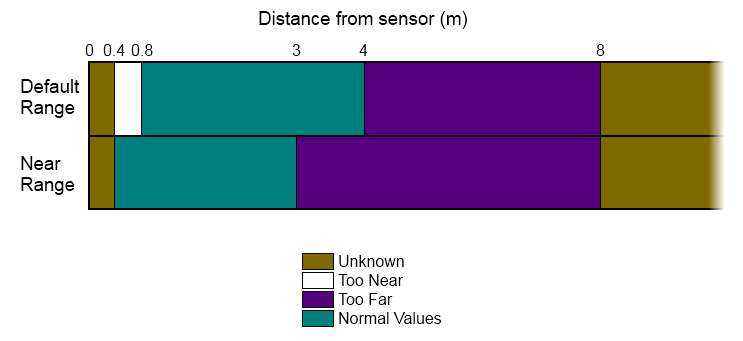
\includegraphics[width=\textwidth]{figures/kinect_sensor_range.png}
\caption{Kinect depth sensor range \cite{microsoft-kinect}.}
\end{figure}


A new generation of smartwatches is leading the way of wearable computing.
These smartwatches are equipped with motion sensors such as
accelerometers, gyroscopes and magnetometers, which are basic components of an
inertial measurement
unit\footnote{\url{http://en.wikipedia.org/wiki/Inertial_measurement_unit}}
(IMU). These sensors can give relatively accurate motion and orientation
information of users' hands at a high frame rate (e.g., the Xsens MTw IMU has
a frame rate of 50Hz~\cite{Ruffieux2013}), and hence, can also be used for gesture input.
The disadvantage of IMUs is that it cannot capture hand shape information.

There is a plethora of new sensors, and they have both pros and cons for hand
tracking and gesture recognition. It is possible to combine different sensors
so that they can complement each other. The sensor technology will continue to
advance, and as a result it is important to make gesture recognition system
that is flexible and generalizable to different feature input. 

I classify
sensors into two categories according to their placement:
environmental and wearable. An environmental sensor is installed at a fixed
position (e.g., the Kinect senor and the Leap Motion Controller); while a
wearable sensor is always available for the user (e.g., smartwatches). I
evaluated my system with two types of sensors from these two categories: the Kinect sensor and the IMU sensor. The Kinect sensor has a built-in microphone array which is
useful for multimodal interaction. Its depth sensor and color camera can be used
for hand shape recognition which is an important part of this work which
combines path and pose gestures in one framework. With the IMUs, I demonstrate
that the framework is generalizable and the two sensors can be used together.

\section{Hand Tracking}
After getting input from the sensor(s), the next step in the pipeline is
tracking the hand(s), i.e., localizing and segmenting hands from the rest of
the input. This step is mainly relevant for camera based sensors, but is trivial
for sensors worn on hands or wrists. 

Common hand tracking methods are based on skin detection~\cite{shin04} or
motion detection~\cite{cutler98}.
Skin detection in an HSV~\cite{bradski98} or YCrCb color space can be relatively
robust and less sensitive to lighting conditions, compared to a RGB color space. However there still can be other materials 
with skin-like colors (such as clothes) that can produce false positives. Skin from other parts of the body can also interfere with hand tracking. 
Shin et at.~\cite{shin04} filter out false positives by considering the skin blob closest to the camera. However this can fail when the hand is close to
the body, generally resulting in the face being detected instead. Methods based on motion-only detection would assume the background is relatively static and there is no motion at
the other parts of the body. In response, I consider skin, motion and closeness
together to compute a probability map for gesture salience.

Marcos-Ramiro et al.~\cite{marcos2013} developed a method of computing hand likelihood maps based on RGB videos
for extracting body communicative cues. They mention that, given a frontal, static camera pointing to the gesturer,  his/her hands are usually the closest
part to the camera, and also move with the highest speed. These characteristics translate to more movement in the image where
the gesturing hand(s) is. As they only use non-stereo RBG images, they can not actually compute the closeness of the movement, and compute the amount
 of motion using optical flow.
My method is very similar to theirs, but we combine both RGB images and depth
 images to compute the gesture salience. We also use depth data to compute the amount of motion which can be computationally less intensive than the optical flow method.

Laptev~\cite{laptev03} introduced the space-time interest points (STIPs) and used them for human
action recognition from movies~\cite{laptev08}. STIPs are points in the video sequence where the image values have
significant local variations in both space and time. His method is an extension of the Harris interest point detector from the spatial domain~\cite{Harris88}
to the spatial-time domain. For each cuboid of interest point, both histograms of oriented gradients (HOG)
and histograms of optic flow (HOF) are computed as feature descriptors. However,
Wang et al.~\cite{wang-spatio-09} compare several space-time feature detectors and descriptors, including STIP, under a common experiment setup for human action recognition and find that dense sampling consistently
outperforms all tested interest point detectors in realistic video settings. They suggest this indicates the limitations of 
current interest point detectors.

Dense sampling is basically computing feature descriptors at regular positions and scales in space and time~\cite{wang-spatio-09}.
It produces a very large number of features, which is more difficult to handle than the relatively sparse number of interest points.
Kone\v{c}n\'{y} and Hagara~\cite{konecny13} also used dense sampling and HOG and HOF
features for gesture recognition. I compared our gesture salience detection and dense
sampling method using the same gesture data set and recognition method, and
my method gives better recognition result.

Another approach to hand tracking is based on 3D body pose estimation and searching for the hand region near the wrist~\cite{song11}.
Skeleton tracking provided by the Kinect Software Development Kit (SDK) gives a relatively robust 3D body pose estimation. The tracking
is based on a body part detector trained from a random forest of a huge number of synthetically-generated poses~\cite{shotton13}. One of its
major strengths is that it does not require an initialization pose. The skeleton
tracking is robust when the whole body is inside the sensor's field of view. In
this case, we use the Kinect skeleton tracking information to provide the
initial estimate of the hand position. However, the hand joint tracking
from the Kinect SDK fails when the hands are close to the body or are moving
fast, especially in the seated mode~\cite{yin13}.
In this case, I use my salience based hand tracking method which
gives a 3.7\% absolute increase in the recognition F1 score when compared with
using the hand joint position from the Kinect SDK based on the ChAirGest
dataset~\cite{Ruffieux2013}.

\cite{sudderth04}

\section{Feature Extraction}
The extraction of low level image features depends on the hand model in use, and
the complexity of the hand model is, in turn,  application dependent.
For a given application, a very coarse and simple model may be sufficient. The simplest model is treating the hand as a
blob and only the 2D/3D location of the blob is tracked. For example, Sharma et
al.~\cite{sharma00} use 2D positional and time differential parameters to track
the hands as blobs, which is sufficient for them to distinguish whether the
hands are doing a point, a contour, or a circle gesture. The PrimeSense NITE
middleware for OpenNI's natural interaction framework also tracks the hand as a
point. It requires the user to do a ``focus'' gesture (``click'' or ``wave'')
to gain control in order to start hand tracking~\cite{primesense-manual}. The
gestures it supports are ``click'' (pushing hand forward), ``wave'', ``swipe
left'', ``swipe right'', ``raise hand candidate'' and ``hand candidate moved''.

However, to make a more generalizable system for natural-like interaction, a
more sophisticated model is required. One step forward is adding fingertip
locations in the hand model as exemplified in~\cite{Oka02, harrison11,
larson11}.
Tracking fingertips is usually sufficient for manipulating objects on the 2D surface. However, for a more rich set of gestures, the one
that also involves 3D manipulation, we may need a more sophisticated
model. For instance, Wang et al. \cite{Wang09} uses a 26 DOF
3D skeletal model in their real-time hand-tracking system with a color glove.
Oikonomidis et al.~\cite{oikonomidis11} also used a parametric 3D model with 26
DOF and 27 parameters. They treat hand pose estimation from markderless visual
observation as an optimization problem and achieved 15Hz frame rate.

Another approach is using an appearance-based model. This means that the model
parameters are not directly derived from the 3D spatial description of the hand.
The hand poses are modeled by relating the appearance of any pose to the 
appearance of the set of predefined, template poses \cite{Pavlovic97}. In
their markless hand-tracking system, Wang et al. \cite{wang11} use efficient
queries of a database of gestures and desktop-specific hand silhouette samples
for pinch/click gesture detection.

In this work, I use a simplified 3D
skeletal hand model for horizontal display interaction where hands are close
to the display surface and can directly manipulate virtual objects.
For communicative gestures, we just need to know the meaning of the gesture instead
of the exact spatial parameters. Hence appearance-based models would be
more suitable which also require less computation, allowing us to achieve
a real-time frame rate of 30Hz.

\section{Gesture Recognition}
Many previous efforts on gesture recognition have focused on one form of
gestures, though here are some work that addressed the problem of handling multiple gesture types in one system.

\subsection{Gesture with Distinct Hand Poses}
One group of prior work focuses on classifying a set of predefined static hand
poses frame by frame. Freeman and Roth \cite{freeman95} use histogram of local
orientations, a precursor of HOG~\cite{dalal05},
for hand pose recognition.
Recognition is based on selecting the feature vector in the training set that is closest to the test feature vector. Suryanarayan et al. \cite{suryanarayan2010} use a volumetric shape
descriptor computed from depth data as the feature vector, and use Support
Vector Machine (SVM) for classification.  I use HOG as a hand pose feature
descriptor but incorporate it in an unified HMM-based framework for both pose
and path gestures.

\subsection{Gesture with Distinct Paths}
Another group of prior work focus on classifying path gestures only, and most of
them used hidden Markov models (HMMs) and its variants to recognize such
gestures~\cite{Starner95, sharma00}.

Starner and Pentland used HMMs to recognize the part of American Sign Language
that uses path gestures~\cite{Starner95}. They collected about 500 sentences of a specific grammar (``personal pronoun, verb, noun, adjective, (the same) personal pronoun'') with a total lexicon of
forty words. No intentional pauses were placed between signs within a
sentence, but the sentences themselves were distinct. Because finger spelling
was excluded and there were few ambiguities in the
vocabulary based on individual finger motion, each gesture word would have a
distinct path.
The feature vector they used includes 8 elements:
each hand's x and y position, angle of axis of least inertia, and eccentricity of bounding ellipse.
They use Gaussian distributions to model the emission probabilities.
When training the HMMs, they used Viterbi training (see Appendix~\ref{app:hmm}
for more details on HMMs) to estimate the initial means and variances of the
output probabilities (after initially dividing the evidence equally among the
words in the sentence).
The initial estimates are fed into a Baum-Welch re-estimator, whose estimates are refined in embedded training.
The techniques they use are very similar to the ones used in speech
recognition given the closer parallel between sign language and speech. In fact,
they were able to use Entropic's Hidden Markov Model TookKit (HTK)\footnote{\url{http://htk.eng.cam.ac.uk/}} directly for all
the modeling and training tasks. Unlike
sign language, gestures for HCI usually are less structured and do not follow a
grammar, hence to learn context-dependent transition and emission parameters will require $O(N^2)$
training examples to cover all possible pairs of gestures for
$N$ gestures.
Our user study indicates that people prefer to give around 5 examples per
gesture, i.e. linear growth with number of gestures. Instead of embedding gesture HMMs in a
sentence, I embed gesture phase HMMs to identify different gesture sub-phases
which is necessary for real-time interaction.
In this way, we learn context-dependent models within a gesture, i.e.,
different gestures may have different pre-stroke and post-stroke phases
depending on their starting and ending points. However, we do not learn
context-dependent models for inter-gesture transition and assume the transitions
between gestures have equal probability.

Sharma et al.~\cite{sharma00} considered natural gestures that are not
bound with syntactical constraints. They examined hand gestures made in a
natural domain, weather narration, and classified three types of
deictic gestures:
\textit{point}, \textit{area}, and \textit{contour}. They also
considered the pre-stroke and post-stroke gesture phases, and used 5 states for
each of the pre-stroke, post-stroke and point HMMs and 6 states for each of the
contour and rest HMMs. The feature vector they use is motion based, and
includes: relative distance of the hand from the face, angle of the arm, angular
velocity etc. Hand poses are not considered. Without considering speech input,
they obtained 69.52\% recognition accuarcy for the three categories of gestures.
Although the deictic gesture is an important category in HCI, it is still
limited for a broader range of applications.

More recently, discriminative models such as
conditional random fields (CRF) and its variants, such as hidden CRF
\cite{wang06} and latent dynamic CRF (LDCRF) \cite{morency07}, have been
applied to gesture recognition with improved recognition results. Morency et al.
\cite{morency07} formulated the LDCRF model that is able to perform sequence labeling and segmentation simultaneously. 
As
discriminative classifiers model the posterior $p(y|x)$ directly, or
learn a direct map from inputs $x$ to the class labels $y$, it is
generally believed that discriminative classifiers are preferred to
generative ones (such as HMMs) for classification problems.
However, one limitation of CRF-based models is that training for these models
is much more computationally expensive and converges much slower than those of
HMMs \cite{lafferty01} because of the larger parameter space to search.
Furthermore, discriminative models can require more training data to reach
lower asymptotic error rates~\cite{ng02}. I applied LDCRF for gesture
classification and gesture phase segmentation.
Compared with my concatenated HMM-based method, LDCRF gives better gesture phase
segmentation result, but lower gesture classification result. The LDCRF model
also takes much longer time to train (18hr on the ChAirGest dataset) compared to
the HMM-based method (which takes 7min). 

\subsection{Different Types of Gestures}
There are some work that addressed the problem of handling multiple gesture
types in one system. Keskin et al. \cite{keskin12} propose a unified framework
to allow concurrent usage of hand gestures, shapes and hand skeletons. Hand gestures are modeled with mixture of HMMs using spectral clustering. Hand shape classification and
hand skeleton estimation are based on randomized decision forests. Hand
gesture classification is active all the time. The framework estimates a set of
posteriors for the hand shape label at each frame, and continuously use these
posteriors and the velocity vector as observation to spot and classify known
gestures. They distinguish gestures with pure motion and pure hand shape by
thresholding the magnitude of the velocity vector. However, they did not mention
handling gestures with distinct hand poses but with arbitrary movement. For this
type of gestures, it will be hard to manually set a velocity threshold to
distinguish them from gestures with distinct paths.

Oka et al. \cite{Oka02} developed a system that
allows both direct manipulation and symbolic gestures. Based on the tracking
result, the system first differentiates the gesture as either manipulative or symbolic 
according to the extension of the thumb. They regard gestures with an extended 
thumb as direct manipulation and those with a bent thumb as symbolic gestures. 
For direct manipulation, the system selects operating modes such as rotate, 
move or re-size based on the fingertips configuration; for symbolic gestures, it 
uses HMM for classification. The way they distinguish manipulative and 
communicative gestures seems to be arbitrary and ``unnatural''. They did that 
probably for the ease of distinguishing it.
My system does not
require an explicit mode switching gesture, and handles the two forms of
gestures seamlessly under one recognition framework. I believe that this can
help reducing users' cognitive load for using the interface, making the interaction more natural.

\subsection{Gesture Spotting}
To distinguish unintentional movements from intentional
movements, a common approach is to use one or two non-gesture HMMs to
provide likelihood thresholds for outlier rejection. For instance, in \cite{yang07}, a weak
universal movement model has been used for adaptive thresholding.
Peng et al. \cite{peng11} argue that using one or two HMMs cannot
effectively reject complex outliers, e.g., when they resemble portions of a
gesture. In addition to a general garbage gesture model, they train several
non-gesture HMM models by automatically identifying and manually specifying
non-gesture models from the training data. This approach is suitable when
identifying dynamic communicative gestures and when the set of the input data is limited. They only test on the
given dataset, but in real life the possible unintentional movements are
limitless and it is not clear how this approach will scale. 

I use gesture phases to distinguish gestures from non-gestures. As explained in
Section~\ref{sec:temporal-model}, every gesture must have a nucleus phase.
My system identifies different gesture phases, and any hand movement that does
not contain a nucleus phase will be treated as a non-gesture.

\subsection{Online Recognition}
Song et al. \cite{song12} extend LDCRF with multi-layered
filtering and a temporal sliding window to perform online sequence labeling and
segmentation simultaneously.
Their approach incurs one to four seconds delay in their
experiments. For real-time interaction, 0.1s is about the limit for having the
user feel that the system is reacting instantaneously. We may relax this response time a
bit, but 1.0s is about the limit for the user's flow of thought to stay
uninterrupted \cite{card91}.  Also they only focus on communicative
gestures and assume no unintentional gestures in the input data. My system
incurs a 0.3s delay.

Fran{\c{c}}oise et al. \cite{francoise11} use hierarchical HMMs to model musical
gestures using motion data from the Wii remote controller, and use fixed-lag
smoothing for real-time recognition and segmentation.
My method is similar to Fran{\c{c}}oise et al.'s, but I consider different
forms of gestures in a single framework.

\subsection{Commercial Systems}
Many commercial gesture recognition systems uses if-then rules based on
heuristics. For example, the Leap Motion
plugin\footnote{\url{https://github.com/hakimel/reveal.js/blob/master/plugin/leap/leap.js}}
for the Reveal.js\footnote{\url{http://lab.hakim.se/reveal-js/#/}} HTML5
presentation framework uses the number of fingers detected and the changes in the $x$ and $y$ coordinates between consecutive
frames to detect swipe and point gestures. While if-then rules could be easy to define for
a small number of simple gestures, it may be hard for more complex gestures.
For example, it may be hard to define a circle gesture using if-then rules and
the rules may conflict with each other.

The gesture interaction provided by the Kinect-based games is
one of the popular ones. Based on the observation of the interaction
available in Kinect games, it seems that the system is only looking for one
gesture (wave) or body pose (the exit
pose\footnote{\url{http://support.xbox.com/en-US/xbox-360/kinect/how-to-use-the-kinect-hub-and-guide}}) at a time, and the rest of the time, 
it is just tracking the hand and the body.

% \begin{lstlisting}
% void LookForGesture() {
%   // Swipe to right
%   if (ScanPositions((p1, p2) => Math.Abs(p2.Y - p1.Y) < SwipeMaximalHeight, // Height
%       (p1, p2) => p2.X - p1.X > -0.01f, // Progression to right
%       (p1, p2) => Math.Abs(p2.X - p1.X) > SwipeMinimalLength, // Length
%       SwipeMininalDuration, SwipeMaximalDuration)) // Duration {
%     RaiseGestureDetected("SwipeToRight");
%     return;
%   }
% 
%   // Swipe to left
%   if (ScanPositions((p1, p2) => Math.Abs(p2.Y - p1.Y) < SwipeMaximalHeight,  // Height
%       (p1, p2) => p2.X - p1.X < 0.01f, // Progression to right
%       (p1, p2) => Math.Abs(p2.X - p1.X) > SwipeMinimalLength, // Length
%       SwipeMininalDuration, SwipeMaximalDuration))// Duration
%         {
%     RaiseGestureDetected("SwipeToLeft");
%     return;
%   }
% }
% \end{lstlisting}

\section{Multimodal User Interfaces}
Bolt's pioneering work in the ``Put That There'' system \cite{Bolt80} 
demonstrated the potential for voice and gestural interaction.  In that system, 
the hand position and orientation were tracked by the Polhemus tracker, i.e.,
the hand was essentially transformed to a point on the screen. The actual hand 
posture did not matter, even if it was not in a pointing shape. The speech also 
followed a rigid and limited command-like grammar. Even though this is early 
work, it provides some insight about the advantages of multi-modal interaction. 
As Bolt summarized in the paper, using pointing gesture allows the use of 
pronouns in the speech, with the corresponding gain in naturalness and economy 
of expression \cite{Bolt80}.

Since then, several multi-modal interaction prototypes were 
developed that moved beyond Bolt's ``Put That There'' system. Cohen et al. 
\cite{Cohen97} developed the QuickSet prototype which is a collaborative, 
multi-modal system running on a hand-held PC using pen and voice as input. They 
used a novel multi-modal integration strategy that allows speech and pen gesture 
to compensate for each other, yielding a more robust system. Rauschert et al. 
\cite{Rauschert02} developed a system called Dialogue-Assisted Visual 
Environment for Geoinformation (DAVE\_G) that uses free hand gestures and speech
as input. They recognized that gestures are more useful for expressing spatial 
relations and locations. Gestures in DAVE\_G include pointing, indicating an 
area and outlining contours. Speech and gesture are fused for commands that need
spatial information provided by the gesture. 

In this thesis, I identify two ways of combining speech and gestures that are
particularly effective for HCI.
In addition to using deictic gestures to provide spatial information as a
complement to speech as in \cite{Rauschert02}, I also use speech as a
complement to manipulative gestures.
based on the user study~\cite{yin10} I
conducted, I observe that manipulative gestures are at times accompanied by
adjectives and adverbs that refine the actions. I demonstrate these two
combinations in a gesture controlled presentation framework I developed.
